% Bottleneck schematic for the article (generated from the normal form with a = -4.834, b = -25.4285, U = 0.1/|b|):
% (a) step per G-iterate across the channel for eps = -1e-5, 0, 1e-5; (b) the 71 iterates of a full passage at eps = 1e-5.
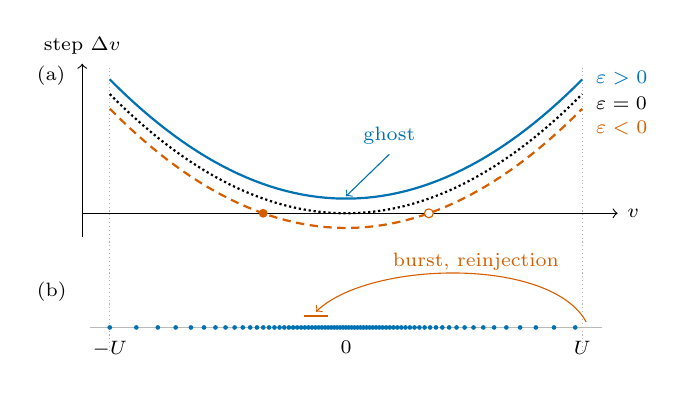
\begin{tikzpicture}[x=1cm, y=1cm, font=\scriptsize]
\definecolor{nfblue}{HTML}{0072B2}\definecolor{nfred}{HTML}{D55E00}
% channel boundaries
\draw[gray!60, densely dotted] (-3,-1.75) -- (-3,1.85); \draw[gray!60, densely dotted] (3,-1.75) -- (3,1.85);
% (a) the step of one iterate
\node[anchor=west] at (-4.05,1.75) {(a)};
\draw[->] (-3.35,0) -- (3.45,0) node[right] {$v$};
\draw[->] (-3.35,-0.3) -- (-3.35,1.9) node[above] {step $\Delta v$};
\draw[nfred, densely dashed, thick, domain=-3:3, samples=60] plot (\x, {1.7*(-0.10947 + 0.89053*(\x/3)^2)});
\draw[black, densely dotted, thick, domain=-3:3, samples=60] plot (\x, {1.7*(0.89053*(\x/3)^2)});
\draw[nfblue, thick, domain=-3:3, samples=60] plot (\x, {1.7*(0.10947 + 0.89053*(\x/3)^2)});
\fill[nfred] (-1.052,0) circle (1.6pt); \draw[nfred, fill=white] (1.052,0) circle (1.6pt);
\node[nfblue, anchor=west] at (3.05,1.72) {$\varepsilon>0$};
\node[anchor=west] at (3.05,1.40) {$\varepsilon=0$};
\node[nfred, anchor=west] at (3.05,1.08) {$\varepsilon<0$};
\draw[<-, nfblue] (0,0.216) -- (0.55,0.75) node[above, nfblue] {ghost};
% (b) the iterates of a full passage
\node[anchor=west] at (-4.05,-1.0) {(b)};
\draw[gray!55] (-3.25,-1.45) -- (3.25,-1.45);
\foreach \p in {(-3.000,-1.45), (-2.663,-1.45), (-2.390,-1.45), (-2.163,-1.45), (-1.970,-1.45), (-1.804,-1.45), (-1.658,-1.45), (-1.530,-1.45), (-1.415,-1.45), (-1.311,-1.45), (-1.217,-1.45), (-1.131,-1.45), (-1.051,-1.45), (-0.978,-1.45), (-0.909,-1.45), (-0.844,-1.45), (-0.784,-1.45), (-0.726,-1.45), (-0.672,-1.45), (-0.620,-1.45), (-0.570,-1.45), (-0.523,-1.45), (-0.477,-1.45), (-0.432,-1.45), (-0.389,-1.45), (-0.347,-1.45), (-0.306,-1.45), (-0.266,-1.45), (-0.227,-1.45), (-0.188,-1.45), (-0.150,-1.45), (-0.113,-1.45), (-0.075,-1.45), (-0.038,-1.45), (-0.001,-1.45), (0.035,-1.45), (0.072,-1.45), (0.109,-1.45), (0.147,-1.45), (0.184,-1.45), (0.222,-1.45), (0.261,-1.45), (0.300,-1.45), (0.340,-1.45), (0.381,-1.45), (0.422,-1.45), (0.465,-1.45), (0.509,-1.45), (0.555,-1.45), (0.602,-1.45), (0.651,-1.45), (0.702,-1.45), (0.755,-1.45), (0.811,-1.45), (0.870,-1.45), (0.932,-1.45), (0.998,-1.45), (1.068,-1.45), (1.142,-1.45), (1.223,-1.45), (1.310,-1.45), (1.404,-1.45), (1.506,-1.45), (1.619,-1.45), (1.743,-1.45), (1.881,-1.45), (2.036,-1.45), (2.211,-1.45), (2.411,-1.45), (2.641,-1.45), (2.911,-1.45)} \fill[nfblue] \p circle (0.85pt);
\node[below] at (-3,-1.5) {$-U$}; \node[below] at (0,-1.5) {$0$}; \node[below] at (3,-1.5) {$U$};
\draw[nfred, thick] (-0.534,-1.3) -- (-0.229,-1.3);
\draw[->, nfred] (3.05,-1.38) .. controls (2.6,-0.55) and (0.3,-0.6) .. (-0.381,-1.25);
\node[nfred] at (1.65,-0.62) {burst, reinjection};
\end{tikzpicture}
